\documentclass[a4paper, 12pt]{article}          % Paper and font size
\usepackage[english]{babel}                     % Language setting

% Set margins
\usepackage[top=2.5cm,bottom=2.5cm,left=2cm,right=2cm,marginparwidth=1.75cm]{geometry}
\usepackage[skip=10pt plus1pt, indent=20pt]{parskip}


% Load useful packages
\usepackage{graphicx}                           % Graphics
\usepackage{amsmath}                            % Math
\usepackage{mathtools}
\usepackage{amssymb}
\usepackage{xcolor}                             % Link color
\definecolor{custom-blue}{RGB}{0,99,166} 
\usepackage{hyperref}
\hypersetup{colorlinks=true, allcolors=custom-blue}
\usepackage[default]{sourcesanspro}             % Load font
\usepackage[T1]{fontenc}                        % Special characters
\usepackage{fancyhdr}                           % Load header, footer package
\usepackage{caption}
\captionsetup{%
  font={footnotesize}, % small font size
  labelfont={bf},      % label in bold, sans-serif
  singlelinecheck=true, % centered single-lined captions
  format=plain,             % indention=1cm,
}

\usepackage{lastpage}                           % Footer note
\usepackage{lipsum}                             % For dummy text
\usepackage{wrapfig}


\pagestyle{myheadings}                          % Own header
\pagestyle{fancy}                               % Own style
\fancyhf{}                                      % Clear header, footer

\setlength{\headheight}{30pt}                   % Set header height
\renewcommand{\headrulewidth}{0.5pt}            % Top line
\renewcommand{\footrulewidth}{0.5pt}            % Bottom line

\fancyhead[L]{
\includegraphics[width=2.5cm]{images/univienna-logo.eps}} % Header left
\fancyhead[C]{}                                 % Header center
\fancyhead[R]{Laboratory: Computational Statistical Mechanics}             % Header right
\fancyfoot[L]{\textcopyright $\,$Tommaso Peritore}         % Footer left
\fancyfoot[C]{}                                 % Footer center
\fancyfoot[R]{\thepage/\pageref{LastPage}}      % Footer right

\usepackage[nottoc]{tocbibind}


%%% Begin document %%%
\begin{document}

\begin{figure}                                  % Include Logo
\flushleft

\includegraphics[width=0.35\textwidth]{images/univienna-logo.eps}
\end{figure}

% Set title, author, date
\title{Report\\Laboratory: Computational Statistical Mechanics}
\author{Tommaso Peritore  \href{mailto:a12446909@unet.univie.ac.at}{a12446909@unet.univie.ac.at}\\Professor: Alessandro Coretti}
\date{2025 Summer Semester, Vienna}

\maketitle                                      
\newpage \tableofcontents

\newpage

\section{Introduction}
The exploration of complex potential energy surfaces (PES) represents a central challenge in statistical mechanics and materials science. These landscapes encode essential information on thermodynamic properties, phase transitions, and the microscopic behavior of matter. However, their high dimensionality and the exponential growth of configurational space render direct exploration computationally challenging, at times impossible. Traditional algorithms have achieved partial success but often face limitations in balancing accuracy, efficiency, and scalability. Often times, alternatively, they focus on one goal at the cost of other information.

Among these methods, the Nested Sampling (NS) algorithm has proven to be a powerful approach for estimating partition functions and thermodynamic quantities by progressively exploring regions of lower energy of a potential. Despite its strengths, NS suffers from inefficiencies when configurational volumes shrink, as well as from correlations between successive configurations that need to be addressed in order to avoid falling into local minima. In parallel, recent advances in generative modeling — particularly the so called denoising diffusion probabilistic models (DM) — have shown remarkable ability to reproduce complex probability distributions and generate uncorrelated samples in high-dimensional spaces.

This project investigates the integration of NS with diffusion models into a mixed algorithm. The aim is to exploit the structured exploration of NS together with the generative power of DM to obtain more efficient sampling of PES, with the potential to reduce computational costs while maintaining accuracy and uniformity of configurations.


\section{Nested Sampling}

The potential energy surface (PES) or energy landscape, describes the energy of a system of particles as a function of the spatial arrangement of the latter \cite{Wales_2004}. In the Born–Oppenheimer approximation - which assumes the coordinates of nuclei of atoms to be stationary while the ones of electrons to be dynamic due to their relative mass difference - the energy landscape gives all the structural and mechanical information of the system. The global minimum of a PES gives the ground state of the system, and depending on the complexity of the surface, many other local minima could exist, indicating a rich variety of stable or metastable configurations of the system, which would be connected via transition states. From the point of view of equilibrium statistical mechanics, the PES describes the free energy of different phases, reflecting the interplay between the potential energy, which is spontaneously decreased in systems, and entropy, which favors phases with larger accessible configuration space volumes, i.e. states obtainable through more configurations. Regions of the PES where the number of accessible configurations sharply declines with decreasing temperature are typically associated with phase transitions, such as freezing or condensation. Understanding these features of the PES is central to many research fields, from exploring dynamic processes like chemical reactions and protein folding, to investigating supercooled liquids and uncovering the microscopic nature of phase transitions.

Computational algorithms have now become essential to the study of PES. However, the complexity of the energy landscapes for most relevant scenarios greatly limits the performances of many algorithms. In fact, if the dimensionality of the PES scales linearly with the dimensionality of the system (the dimensions of the PES are in fact the degrees of freedom of the system), the configurational space volume scales exponentially with the system size. And also the number of minima are thought to scale exponentially \cite{Hoare1979}. The methods introduced so far are vast, often specific to analyzing certain details or features of the PES. In the specific scenario of the study of materials, the difficulty lies in the necessity to explore all possible regions of the PES to obtain relevant information on the free energy, rather than limiting the study to minima. This task is, as stated above, computationally demanding. 

And that is where the method we took into consideration comes into play. Nested sampling (NS) was originally introduced by Skilling \cite{Skilling2004, Skilling2006, Skilling2009} in the field of applied probability and inference, to sample sharply peaked probability densities in high-dimensional spaces. In statistical physics, this translates to estimating the partition function and thermodynamic quantities. In NS one writes the partition function as an integral over configuration-space volume below each energy level, and then samples states in order of decreasing energy. As Pártay et al. note , NS addresses the problem of finding a suitable set of sample points for the estimation of thermodynamical functions which can be essentially related to the energy of the sample points and its relative density of microstates \cite{Partay2021NestedSampling}. The key idea of the algorithm is to automatically coarsely sample high-energy (low-weight) regions and progressively refine sampling in the small-volume, low-energy regions where most statistical weight lies. In other words, NS focuses computational effort on the part of the energy landscape that contributes most to the partition function. 


% do I need to add illustrations??? %%%%%


\subsection{The algorithm}
In this section we will explicitly walk through the algorithm of Nested Sampling, as it was presented in \cite{Partay2021NestedSampling} focusing on the aspects of the algorithm that were implemented in our work. In fact, if the core idea of the algorithm is one, different choices can be made on some aspects of the process to better fit different scenarios.
%\begin{wrapfigure}{r}{0.5\textwidth}
%   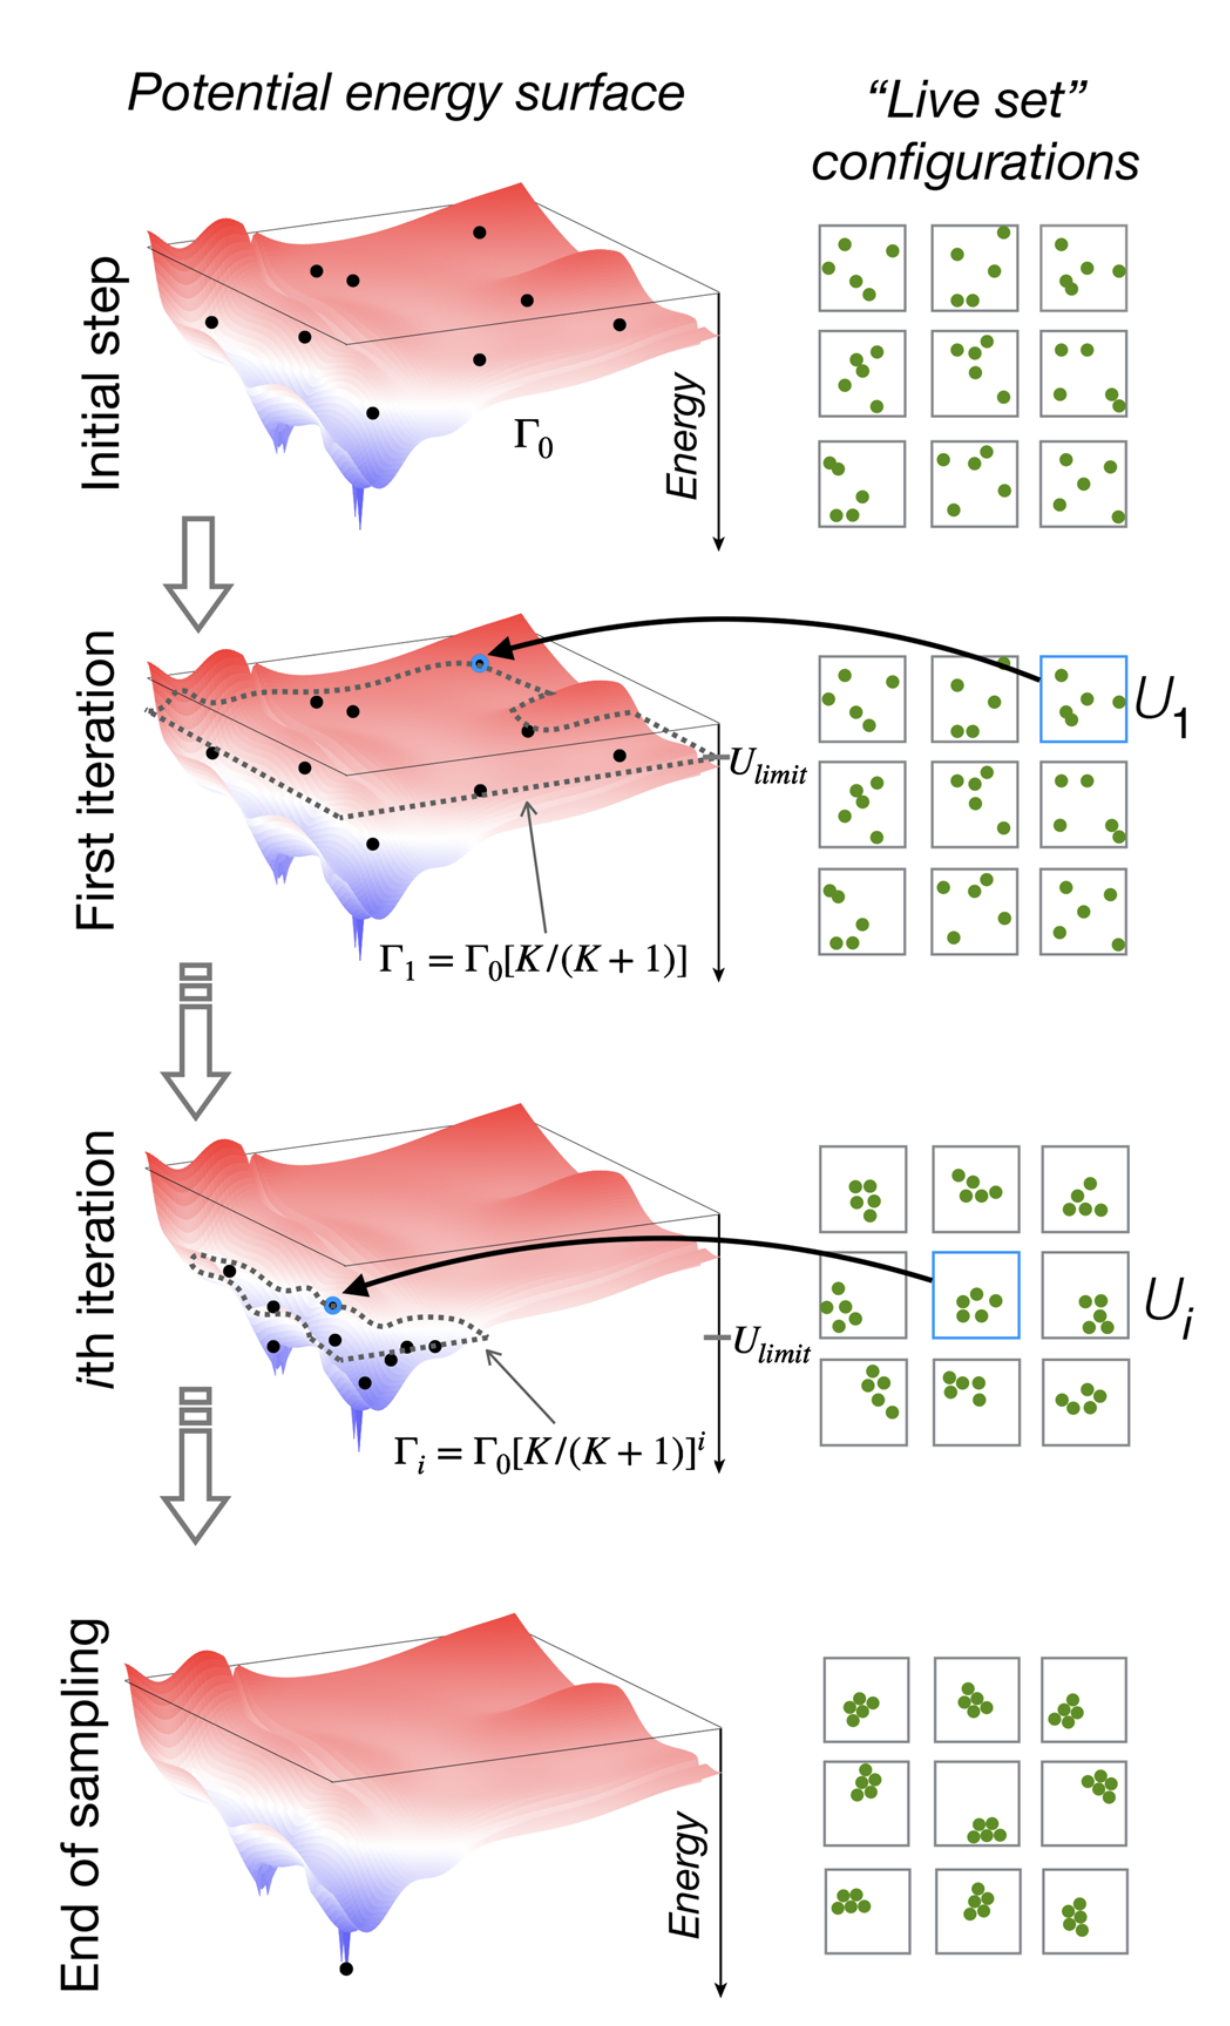
\includegraphics[width=0.95\linewidth]{images/NSAlgorithm.png}
%   \caption{Illustration of the nested sampling algorithm, showing several steps of the iteration. Panels on the left-hand side represent the PES (the vertical axis being the potential energy, while the other two axes representing the phase-space volume). Black dots on the landscape demonstrate the members of the live set (in this illustration K = 9) uniformly distributed in the allowed phase space corresponding atomic configurations (assuming constant volume sampling) are shown in the right-hand side panels. In the middle two panels, the samples with the highest energy are shown by blue, with the corresponding energy contour illustrated by a dotted line. Image from \cite{Partay2021NestedSampling}.}
%   \label{img:ns_alg_sketch}
%\end{wrapfigure}
The initialization happens through the generation of $K$ uniformly distributed (in the space of positions) random configurations called "live set". Each configuration is the vector needed to define a state of our atomic system, i.e. if we're considering a single particle on a two-dimensional potential, this would be a set of $(x,y)$, making the PES live in $\mathbb{R}^3$; for $N$ particles in space the energy function becomes of the form $U(\mathbf{x}):\mathbb{R}^{3N}\rightarrow\mathbb{R}$. Each one of the $K$ points will have its associated energy. The algorithm can now find the point that yields the highest energy, save this value, say as $U_{limit}$ and delete the point from the live set. Now the algorithm generates a new point withing the energy threshold $U_{limit}$, and calculates once again the highest energy to then repeat the iteration. In this way, each new set is a uniform distribution of configurations that respect the condition of having $U<U_{limit}$, exploring regions of the PES with progressively lower energy but always keeping the property of uniform sampling, thus avoiding to bias the exploration on local minima. 

One aspect that we have thus far overlooked is how to actually generate new configurations at each step of the iteration. This can in fact be done in many different ways. Our implementation of the algorithm used one strategy in particular. 

\subsection{Points generation}
To make the pool of live points explore the energy surface descending its slopes a way is needed to generate configurations that are progressively lower in the highest value of energy that they take. To achieve this, from our initial configuration, we substitute the point of highest energy with an existing point (effectively duplicating it). On the whole set of live points is applied a random walk step of definite length, thus shuffling the set, but accepting only those steps that move the points within the highest energy previously reached. This is in a way a random step within a border. Then finally we can obtain the new maximum energy and the point that achieves it to repeat the generation of new live set once until reaching a minima.

However, if at the beginning this is surely going to be a very successful algorithm, as the configuration volume shrinks, many steps are likely to be rejected. To fix this issue we have introduced a number of steps to be made with the same energy threshold, in order to avoid having configurations that almost do not evolve. The details of this decorrelation procedure are not entirely clear. If on one hand it is evident, as previously mentioned, that we want our configurations to be uniform at all times, and in this goal decorrelating the positions does help, on the other hand we were not able to analyze the amount of steps required to really decorrelate. 

\subsection{Implementation and potential} \label{subsec:impl_pot}
For our use, we've implemented the algorithm entirely as it was presented in the paper, with the choice of live points generation scheme that was presented above. As a benchmark of our implementation of the algorithm, we used the simple two-dimensional potential well 
\begin{equation} \label{eq:pot}
    U(x,y) = \varepsilon \left(
    c \left(x^2 - 1 \right)^2 
    + \left(x - y\right)^2 
    + d \left(x + y\right)
\right) 
\end{equation}
with $\varepsilon$, $c$ and $d$ being parameters of the well. Some contour levels are shown in fig. \ref{fig:pot} together with a 3D visualization. This energy function is known and easy to work with, also in terms of computational evaluation of the energy value given a point. Its minima are known to be $\left(1,1+d/2\right)$ and $ \left(-1,-1+d/2\right)$. 

\begin{figure}[ht]
    \centering
    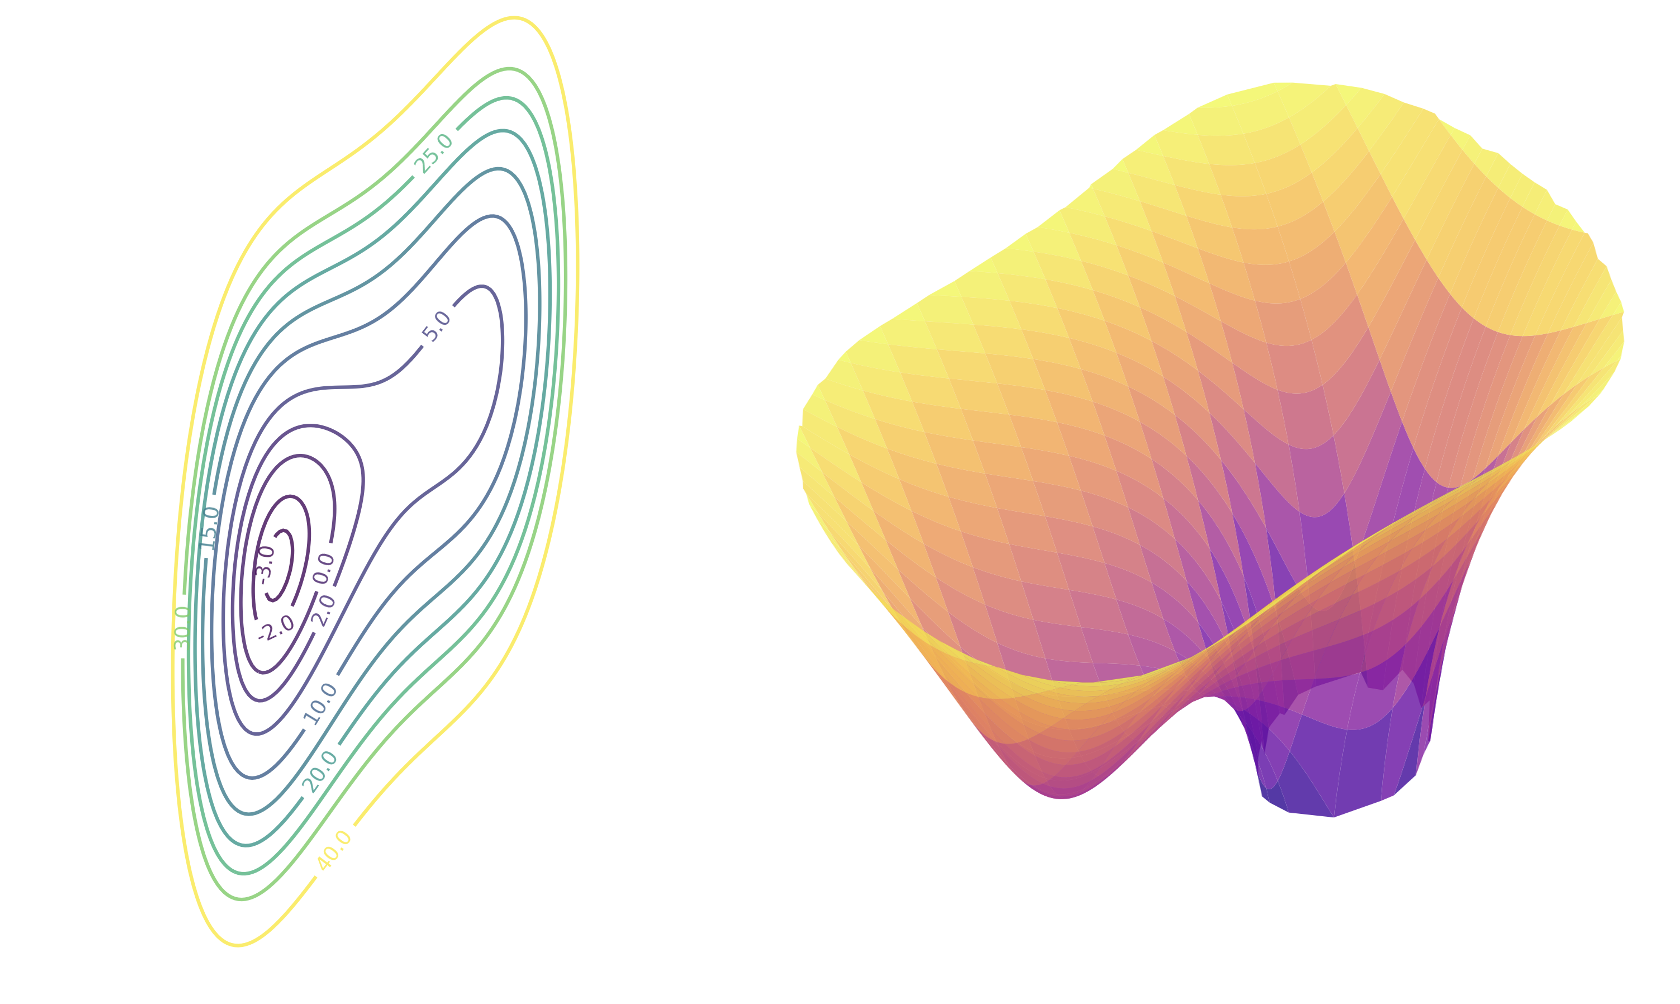
\includegraphics[width=0.85\linewidth]{images/pot.png}
    \caption{Contour levels of the benchmark potential and 3D visualization.}
    \label{fig:pot}
\end{figure}


 
\section{Diffusion Models}

Diffusion models are a class of generative models that have recently achieved remarkable success in producing high-quality samples in domains such as image synthesis, audio generation, and molecular modeling. These models are inspired by nonequilibrium thermodynamics and operate by simulating a gradual transformation of data into noise and then learning how to reverse this process to recover the original data.

At the heart of a diffusion model is a two-stage process:
\begin{enumerate}
    \item Forward (diffusion) process, a Markovian process that incrementally adds Gaussian noise to the data over a series of time steps, eventually transforming the data into pure noise. The noise level increases over time, and the process is designed to be simple and fully known, that is the schedule used to add noise is predefined. 
    \item Reverse (denoising) process, which learns to gradually remove the noise added during the forward process. Since this is generally intractable to compute exactly, it is approximated using a deep neural network trained to predict either the original data, the noise, or the clean sample at each step.
\end{enumerate}

Diffusion models offer several appealing properties. Unlike Generative Adversarial Networks (GANs), they are trained with a simple and stable likelihood-based objective, often derived from variational inference. Furthermore, they can model complex distributions without suffering from mode collapse, a common issue in GANs.

A prominent variant of diffusion models, which is the version we have taken up as the starting point of our model, is the Denoising Diffusion Probabilistic Model (DDPM), which was introduced by Ho et al. in 2020 \cite{Ho2020}. It uses a fixed variance schedule for the forward process and trains a neural network to denoise samples at each step of the reverse process. Since then, many improvements and extensions have been proposed, including conditional diffusion models, improved sampling strategies, and methods to accelerate the sampling process.

Let us examine the details of the model, analyzing also the modifications we have introduced to better fit our use case.

\subsection{Forward process}

\begin{figure}[h]
    \centering
    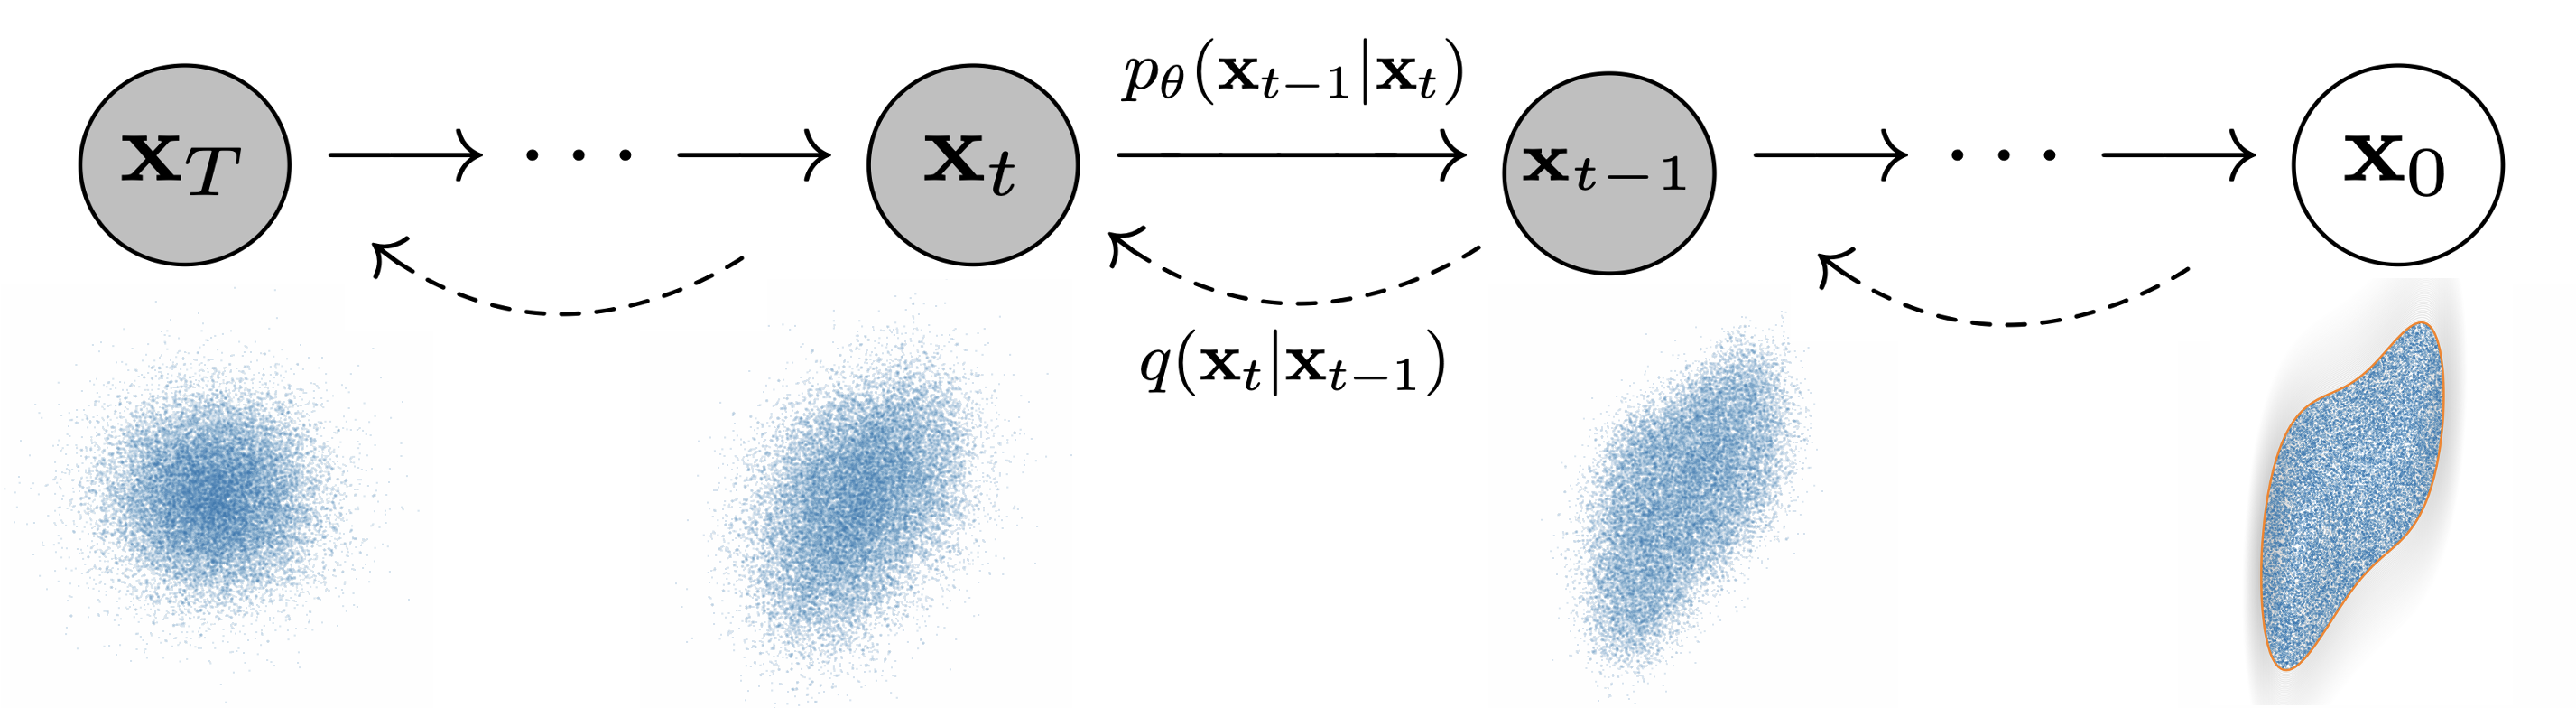
\includegraphics[width=0.85\linewidth]{images/forward_pr.png}
    \caption{Representation of the processes utilized in the diffusion model. The dashed arrows represent the steps of the forward process achieved through the distributions $q(\mathbf{x}_t | \mathbf{x}_{t-1})$, applied from right to left, while the reverse process is achieved by applying from left to right the learned distributions $p_\theta(\mathbf{x}_{t-1} | \mathbf{x}_t)$.}
    \label{fig:forward_pr}
\end{figure}

The forward process is defined as a fixed Markov chain that adds Gaussian noise to a data sample $\mathbf{x}_0$ over $T$ discrete time steps, producing a sequence $\{\mathbf{x}_1, \mathbf{x}_2, \ldots, \mathbf{x}_T\}$ of progressively more noisy data, called latent variables, as seen in the above fig. \ref{fig:forward_pr} from right to left. At each step $t$, noise is added according to a variance schedule $\beta_t$, making the transition distribution, that is the distribution at time $t$ coming from time $t-1$ a Gaussian as follows:
\begin{equation}
    q(\mathbf{x}_t | \mathbf{x}_{t-1}) = \mathcal{N}(\mathbf{x}_t; \sqrt{1 - \beta_t} \mathbf{x}_{t-1}, \beta_t \mathbf{I}).
\end{equation}
where the noise added is centered in the previous sample $\mathbf{x}_{t-1}$ rescaled by a factor $\sqrt{1-\beta_t}$ with a variance of $\beta_t$. Thus the distribution of the samples, from the initial data $\mathbf{x}_0$ to the final step $T$, is obtained via a combination of these steps as
\begin{equation}
    q(\mathbf{x}_{1:T} | \mathbf{x}_0) \coloneqq \prod^T_{t=1} q(\mathbf{x}_t | \mathbf{x}_{t-1}).
\end{equation}
Intuitively, this gradually perturbs the original data with noise until, at the final step $T$, the data is nearly indistinguishable from pure Gaussian noise. It can actually be shown how the step $T$ for this defined variance schedule reaches a perfect Gaussian distribution $\mathcal{N}(0,\mathbf{I})$. 

The fixed schedule allows for a particular characteristic of the forward distribution, that of being available for sampling in closed form. In fact we can write
\begin{equation}
    q(\mathbf{x}_t | \mathbf{x}_0) = \mathcal{N}(\mathbf{x}_t;\sqrt{\bar{\alpha}_t}\mathbf{x}_0 , (1-\bar{\alpha}_t)\mathbf{I}),
\end{equation}
having defined
\begin{equation}
    \bar{\alpha}_t = \prod_{s=1}^t (1 - \beta_s)
\end{equation}
calculating the cumulative effect of all steps from $0$ to $t$ without actually having the intermediate samples $\mathbf{x}_i\;i\in(0,t)$.

It is important here to point out that as we've presented things, the fact that the process is fixed, thus not requiring learning any parameter, is an ingredient that is not required but essential to make things workable with. It is in fact how this process was presented in its original paper, and only later will learning the forward process be proposed as an alternative, as was happened, for example, in \cite{Nichol2021ImprovedDDPM}.

\subsection{Reverse process}

The goal of the diffusion model is to learn the reverse process, i.e. inverting the addition of noise applied in the forward process to be able to gradually remove noise (denoising) to recover $\mathbf{x}_0$ starting from the noisy $\mathbf{x}_T$. This reverse chain is modeled as a Gaussian with learnable parameters: 
\begin{equation} \label{eq:rev_def}
p_\theta(\mathbf{x}_{t-1} | \mathbf{x}_t) = \mathcal{N}(\mathbf{x}_{t-1}; \boldsymbol{\mu}_\theta(\mathbf{x}_t, t), \boldsymbol{\Sigma}_\theta(\mathbf{x}_t, t)),
\end{equation}
where $\boldsymbol{\mu}_\theta$ and $\boldsymbol{\Sigma}_\theta$ are the functions that, depending on the time and distribution we're looking to obtain, $\mathbf{x}_t$, give the mean and variance learned in the neural network through the parameters $\theta$. 

The full reverse process is the joint distribution defined as 
\begin{equation}
    p_\theta(\mathbf{x}_{0:T}) = p(\mathbf{x}_T) \prod^T_{t=1}p_\theta ( \mathbf{x}_{t-1}|\mathbf{x}_t),
\end{equation}
starting from the Gaussian $p(\mathbf{x}_T) = \mathcal{N}(\mathbf{x}_T;\boldsymbol{0},\mathbf{I})$. By learning the parameters, the network is trained to approximate the true reverse distribution of the forward noising process.

\subsection{Training objective}

Now that the ingredients of the process have been presented, we get to the essential ingredient needed for training: the definition of the loss. This is the function that allows the network to learn, and as is usually done in these scenarios, training happens by optimizing the variational bound on negative log likelihood,
\begin{equation}
    \mathbb{E} \left[ -\log p_\theta(\mathbf{x}_0) \right].
\end{equation}
This function, in fact, gives an evaluation of how close the learned distribution is to the actual original sample. 

However, as it is now, this expectation value is dependent on all possible trajectories taken by our sample through the denoising process, and as such, it is impossible to compute. Thus, the following subsection will be used to make sense of a simplification of the objective essential for it to be usable within the model that was presented in the original paper \cite{Ho2020}.

\subsubsection{Simplifying the loss function}
First off, the negative log likelihood can be bounded by introducing a dependence on the schedule of the forward process and introducing a form of Jensen's inequality, usually applied on these kinds of distributions:
\begin{equation} \begin{split}
    \mathbb{E} \left[ -\log p_\theta(\mathbf{x}_0) \right] &= \mathbb{E} \left[ -\log \left[ \int dx_{1:T} q(\mathbf{x}_{1:T}| \mathbf{x}_0)p(\mathbf{x}_T)\prod_{t=1}^T \frac{p_\theta(\mathbf{x}_{t-1} | \mathbf{x}_t)}{q(\mathbf{x}_t | \mathbf{x}_{t-1})}\right]\right]\\
    & \leq \mathbb{E} \left[ -\log \left[p(\mathbf{x}_T) \prod_{t-1}^T \frac{p_\theta(\mathbf{x}_{t-1}|\mathbf{x}_t)}{q(\mathbf{x}_t | \mathbf{x}_{t-1}}\right]\right] \\
    & \leq \mathbb{E} \left[ -\log p(\mathbf{x}_T) - \sum_{t=1}^T \log \frac{p_\theta(\mathbf{x}_{t-1} | \mathbf{x}_t)}{q(\mathbf{x}_t | \mathbf{x}_{t-1})} \right] \; =: \;  L,
\end{split} \end{equation}
where the last step thus has defined the loss function.

Now we will use a standard function for comparing distributions, the Kullback-Leibler divergence:
\begin{equation}
    D_{KL} (q\|p) = - \int q(x)\log\frac{p(x)}{q(x)}dx,
\end{equation}
through which the loss can be written as 
\begin{equation} \begin{split}
    L &= \mathbb{E} \left[ D_{KL}\left( q(\mathbf{x}_T | \mathbf{x}_0)\| p(\mathbf{x}_T) \right) + \sum_{t>1}D_{KL}\left( q(\mathbf{x}_{t-1} | \mathbf{x}_t, \mathbf{x}_0) \| p_\theta(\mathbf{x}_{t-1} | \mathbf{x}_t) \right) - \log p_\theta(\mathbf{x}_0 | \mathbf{x}_1) \right]\\
    &=  L_T + \sum_{t>1}L_{t-1} + L_0 .
\end{split} \end{equation}
The first term isn't learnable since we have fixed the schedule $\beta_t$, and the last is also ignored. 
Now to compare the reverse with the forward process we can express the forward by conditioning on $\mathbf{x}_0$ as
\begin{equation}
    q(\mathbf{x}_{t-1}|\mathbf{x}_t,\mathbf{x}_0) = \mathcal{N}(\mathbf{x}_{t-1}; \tilde{\boldsymbol{\mu}}_t(\mathbf{x}_t,\mathbf{x}_0),\tilde{\beta}_t\mathbf{I}),
\end{equation}
having defined
\begin{equation} \label{eq:subst}
    \tilde{\boldsymbol{\mu}}_t(\mathbf{x}_t,\mathbf{x}_0) := \frac{\sqrt{\bar{\alpha}_{t-1}}\beta_t}{1-\bar{\alpha}_t}\mathbf{x}_0 + \frac{\sqrt{\alpha_t}(1-\bar{\alpha}_{t-1})}{1-\bar{\alpha}_t}\mathbf{x}_t \;\; \mathrm{and} \;\; \tilde{\beta}_t := \frac{1-\bar{\alpha}_{t-1}}{1-\bar{\alpha}_t}\beta_t
\end{equation}
and also defining $\alpha_t := 1-\beta_t$ and $\bar{\alpha}_t := \prod_{s=1}^t\alpha_s$. This allows to directly compare the mean values of the Gaussian distribution at random time steps with the learned Gaussian mean transitions of the reverse process by suggesting a parametrization of the loss function directly through these means. A choice made by the original authors is also to leave the variance of the reverse process unlearned, i.e. $\boldsymbol{\Sigma}_\theta(\mathbf{x}_t,t) = \sigma_t^2\mathbf{I}$  (with a fixed $\sigma$ which we will take as $\sigma^2_t = \beta_t$) which they have experimentally found to yield good results while greatly simplifying the number of learnable parameters. This makes the reverse process (defined in eq. \ref{eq:rev_def}):
\begin{equation}
    p_\theta(\mathbf{x}_{t-1} | \mathbf{x}_t) = \mathcal{N}(\mathbf{x}_{t-1}; \boldsymbol{\mu}_\theta(\mathbf{x}_t, t), \sigma^2_t\mathbf{I})
\end{equation}
The above observations allow us to rewrite the missing term of the loss as
\begin{equation}
    L_{t-1} = \mathbb{E} \left [ \frac{1}{2\sigma^2_t} || \tilde{\boldsymbol{\mu}}_t(\mathbf{x}_t,\mathbf{x}_0) - \boldsymbol{\mu}_\theta (\mathbf{x}_t,t) || ^2 \right] + C
\end{equation}
where we have left in the constant $C$ everything that doesn't depend on the parameters $\theta$. 

This is already a step forward as we have now a loss dependent on the learned mean, rather than on the distributions. However, a further simplification can be made by noting that our choice of fixed variance schedule and of progressive Gaussian noise dependence from one step to the next in the forward process allows us to express the sampling of any time $t$ in closed form from $\mathbf{x}_0$:
\begin{equation}
    q(\mathbf{x}_t | \mathbf{x}_0) = \mathcal{N}\left(\mathbf{x}_t ; \sqrt{\bar{\alpha}_t}\mathbf{x}_0 , (1-\bar{\alpha}_t)\mathbf{I} \right).
\end{equation}
Thus the step $\mathbf{x}_t$ can be easily obtained by sampling $\boldsymbol{\epsilon} \sim \mathcal{N}(\mathbf{0},\mathbf{I})$ and computing:
\begin{equation} \label{eq:x_t}
    \mathbf{x}_t = \sqrt{\bar{\alpha}_t} \mathbf{x}_0 + \sqrt{1 - \bar{\alpha}_t} \boldsymbol{\epsilon}.
\end{equation}
In these terms, the forward process posterior mean $\tilde{\boldsymbol{\mu}}_t$ can be made, through substitution of the inverse of eq. \ref{eq:x_t} in eq. \ref{eq:subst}, to be
\begin{equation}
    \tilde{\boldsymbol{\mu}}_t = \frac{1}{\sqrt{\alpha_t}}\left(\mathbf{x}_t (\mathbf{x}_0,\boldsymbol{\epsilon}) - \frac{\beta_t}{\sqrt{1-\bar{\alpha}_t}}\boldsymbol{\epsilon} \right).
\end{equation}
This reveals that the loss asks that the $\boldsymbol{\mu}_\theta$ predict the right-hand side of the above equation, given $\mathbf{x}_t$. Since this is readily obtained in the model, we can parameterize through an error, defining
\begin{equation}
    \boldsymbol{\mu}_\theta(\mathbf{x}_t, t) = \frac{1}{\sqrt{\alpha_t}}\left(\mathbf{x}_t - \frac{\beta_t}{\sqrt{1-\bar{\alpha}_t}}\boldsymbol{\epsilon}_\theta(\mathbf{x}_t,t)\right),
\end{equation}
where the network predicts $\boldsymbol{\epsilon}_\theta(\mathbf{x}_t, t)$, an estimate of the noise that should have been introduced to be able to sample the timestep $t$ in the forward process. 

Going back with this result to the loss, we have obtained that
\begin{equation}
    L_{t-1} - C = \mathbb{E} \left[ \frac{\beta_t^2}{2\sigma_t^2\alpha_t(1-\bar{\alpha}_t)} \| \boldsymbol{\epsilon} - \boldsymbol{\epsilon}_\theta \left(\sqrt{\bar{\alpha}_t}\mathbf{x}_0 + \sqrt{1-\bar{\alpha}_t} \boldsymbol{\epsilon},t\right) \|^2  \right]
\end{equation}
where apart from the sample distribution $\mathbf{x}_0$, the model loss only needs to predict the error introduced to sample $\mathbf{x}_t$ as in eq. \ref{eq:x_t}.

The coefficient obtained in front of the norm is also found to have a small impact on the sample quality, as well as being a bit more difficult to implement. Thus, in the original paper, it was found that the best parametrization of the reverse process to obtain treatable and accurate loss evaluation was
\begin{equation}
    L_{\mathrm{simple}}(\theta) := \mathbb{E}_{t,\mathbf{x}_0,\boldsymbol{\epsilon}} \left[ \| \boldsymbol{\epsilon} - \boldsymbol{\epsilon}_\theta \left(\sqrt{\bar{\alpha}_t}\mathbf{x}_0 + \sqrt{1-\bar{\alpha}_t} \boldsymbol{\epsilon},t\right) \|^2 \right].
\end{equation}

Having obtained this closed form for the loss, the training happens through optimization of random steps using stochastic gradient descent.

\subsection{Sampling procedure}

To generate new data, sampling begins with a noise vector $\mathbf{x}_T \sim \mathcal{N}(\mathbf{0}, \mathbf{I})$ and applies the learned reverse process iteratively to produce $\mathbf{x}_{T-1}, \mathbf{x}_{T-2}, \ldots, \mathbf{x}_0$. Each step involves sampling from the Gaussian distribution parameterized by the network output:
\begin{equation}
    \mathbf{x}_{t-1} \sim p_\theta(\mathbf{x}_{t-1} | \mathbf{x}_t).
\end{equation}
After $T$ steps, the result $\mathbf{x}_0$ is a sample from the learned data distribution. 

\subsection{Adjustments to the model}
Our use of the model is of course connected with the exploration of the energy surface. In particular, we want our model to help us generate configurations of a given energy, that have to be randomly and uniformly distributed within the configurational volume. This could be an improvement to the nested sampling algorithm as once the model is trained, it readily generates configurations that are completely uncorrelated with the previously generated or with the ones used for training. Nonetheless, more details on this will come in \ref{sec:mixed_alg}, but the adjustments to the model were done to prepare it for this use case.
Not introduced in the original paper, but rather in \cite{Nichol2021ImprovedDDPM}, is the idea to condition the network. In our case, we want the model to generate configurations of a given energy, thus it comes natural to give to the model in phase of training, on top of the configurations, which make the sample $\mathbf{x}_0$ we would like to replicate, also the energy of that sample. In a way this is already done in the original paper, where time, as the measure of distance from the final gaussian sample $\mathbf{x}_T$ to the initial $\mathbf{x}_0$, is embedded in the model as one more node of input on top of the positions required. Thus similarly for the energy we can simply add a layer of input in the network structure, so that on top of the $K$ live points and the time evolution parameter $t$, an input is also made of the energy threshold that stays the same within the whole time span of the process.

The network's structure is made up of a $5$ sets of a linear transformation and a ReLu activation function one after the other. The internal linear transformations are set with input and output size of $64$ nodes. 

 
\section{Mixed algorithm implementation} \label{sec:mixed_alg}

We have thus far introduced the foundations of our work, the ingredients we need to combine. In fact, our goal is to make a tool to generate, possibly more efficiently, uniformly distributed and independent configurations under a certain value of energy. This, as said above, is in the hopes of improving the nested sampling algorithm through the exploit of the diffusion model.

The initialization of the algorithm works the same way as what we presented for the nested sampling algorithm. We start from a set of $K$ points in the domain of the energy function, in the case of the potential well presented in \ref{subsec:impl_pot}, this is $K$ points in $\mathbb{R}^2$, which make up what we call our live set. We find the maximum energy reached by these points, to then have them shuffled around the domain while keeping them within the maximum energy. After a few iterations of this procedure we will have a live set, called $\mathbf{x}_1$ within a certain $U_1$. At this point, this live set is used to train our diffusion model (with or without conditioning, i.e. passing also the value of $U_1$ as input to the model, we will get to the differences later). With the model trained we can use it to generate a number of new points that make up an intermediate pool, which we call $\mathbf{x}_1^p$. Now, one at a time, we will use points from this generated pool to substitute the points of highest energy from the sampled used to train $\mathbf{x}_1$. That is, we find the point $(x,y)\in\mathbf{x}_1$ that has the highest energy and substitute it with one $(x^p,y^p)\in\mathbf{x}_1^p$, until all points of the pool have been used up. Before the substitution we do need to check that the point of the pool is actually within the maximum energy. The latter will be $U_1$ for the first substitution but will be then updated to help following substitutions in being more effective. Another point to note is that an important aspect to look into for the performance of this mixed step is the number of points in the generated pool, which does not need to be $K$, and in fact determines how much the mixed routine relies on the model or rather on the nested sampling part of the algorithm. 

Once all the points from the pool have been used up, the first complete step of the mixed routine is done. Now we could right away train a new model but since most of the points present should be from that pool, we let our new live set through a few nested sampling steps. Here again the choice of how many steps is crucial for the behavior of the algorithm: letting it take many steps will make it so that the mixed algorithm is still heavily reliant on the NS part, while reducing this number lets the model generations do most of the work taking our live set down the potential well. Then the new live set, $\mathbf{x}_2$ will be used to train the new model, so as to generate the new pool $\mathbf{x}_2^p$ which will again replace one by one the points of the live set. Iterating this procedure allows us to combine the work of these two tools to enhance the nested sampling algorithm. In fact, after training, it is without the expense of random walks that we have access to uncorrelated points that used one by one take the live set quickly down the potential. 

\subsection{Critical aspects}
From what we presented above come certain critical aspects that could mine the effectiveness of this mixed routine, or need to be tweaked to make the implementation of the diffusion model competitive against the NS algorithm by itself.

First off is the problem of rejection of points from the generated pool. That is, when we train the model on a live set within a certain energy threshold, it correctly generates points uniformly distributed in that position space volume. Similarly to what we discussed with the NS algorithm, as the volume shrinks, swapping positions with new generated ones, it becomes more likely that more positions of the pool fall outside the contour line of the new energy threshold. In the NS algorithm such steps (taking a point outside the contour) would be ignored, but now this is a greater expense if the cost of sampling from the model is significant. Our approach was to avoid generating too many points from a single train to limit the number of rejections before generating from a new model trained on tighter contours. The fine tweaking of this aspects was addressed by monitoring the acceptance rate throughout the use of the generated pool points. Ultimately, the adjustment has to mirror the interplay of cost between training and generating points from the model and applying the random walk steps of the nested sampling. 

Another critical aspect is that the generation of points from the trained model does not assure that the points be within the contour of the energy provided upon training. In fact, the model is not guaranteed (and actually never does) to learn exactly the contour and thus to place all points inside of it. Thus the above problem of rejection is true from the beginning, where already some points will be outside the contour of the initial energy threshold. To improve on this, we did experiment a way to further help the model to learn the contour. After the first full step of the mixed algorithm, upon training the second time our model, we provide not only the last live set and its maximum energy, but also the first live set and its energy. And so forth the third training will receive three live sets and their energies. This is in the hopes that providing the model with the evolution of the contour lines with the decreasing energy will help it to understand better the shape of the contour. The effectiveness of this approach will be presented in the section of Results \ref{sec:results}. 

Actually, also the fact of conditioning itself needs to be tested. If doing training with more live sets simultaneously (as presented above) naturally suggests to provide their relative energies for the model to distinguish them, when training with a single set it is not obvious that providing the energy as another input might help the model. 

% still missing illustrations: might have to rethink the mixed alg from the presentation


\section{Results} \label{sec:results}

% aspects to explore : effect of # of diffusion steps on quality of data (first accuracy then density)
% mixed alg : cond vs no cond ; evaluation: time, en call, iterations

All the material used and produced for the project can be found at the dedicated \href{https://github.com/tommasoperitoree/CSM_Lab}{GitHub page}. This includes all the code written for the project or taken from the articles cited above, as well as more material than what we can show here; we will thus refer to the specific location in the repository to find additional evidences of the results provided.

\subsection{Diffusion model evaluation}

Before attempting to put to use the diffusion model in the mixed algorithm, we looked into its performances by itself. In the project's GitHub, under ./resources/forward$\_$process/ animations of the forward process of noising can be found for different contour levels. Furthermore, under ./resources/nested$\_$sampling$\_$configs/ one can find the results of the nested sampling algorithm working by itself to take the live set down to the potential's minima.

The diffusion process is characterized by the schedule, i.e. the set of $\beta_t$ for $t\in[0,T]$. This is a double dependence: firstly how big $T$ is means how fine grained we will allow our schedule to be through the division of the whole process in more or less intermediate steps; secondly, the absolute values of $\beta_t$ affects how much noise we introduce at every step of the procedure. We have mentioned that in any case the noising process takes our data to be distributed normally at the last step, but these two details decide respectively how many intermediate steps there are and how abrupt the change will be from one to the other. The paper presenting the DM \cite{Ho2020} takes values of $\beta\in[10^{-4},0.02]$ which we kept also for our implementation. However, we did explore different number of diffusion steps $T$. We thus trained the model to replicate certain contour levels and then looked at the generated pool, comparing it with the actual contour line, to see what percentage of the generated points were actually within the threshold. In fig. \ref{fig:accur_1} is one example of the results obtained. 

\begin{figure}[ht]
    \centering
    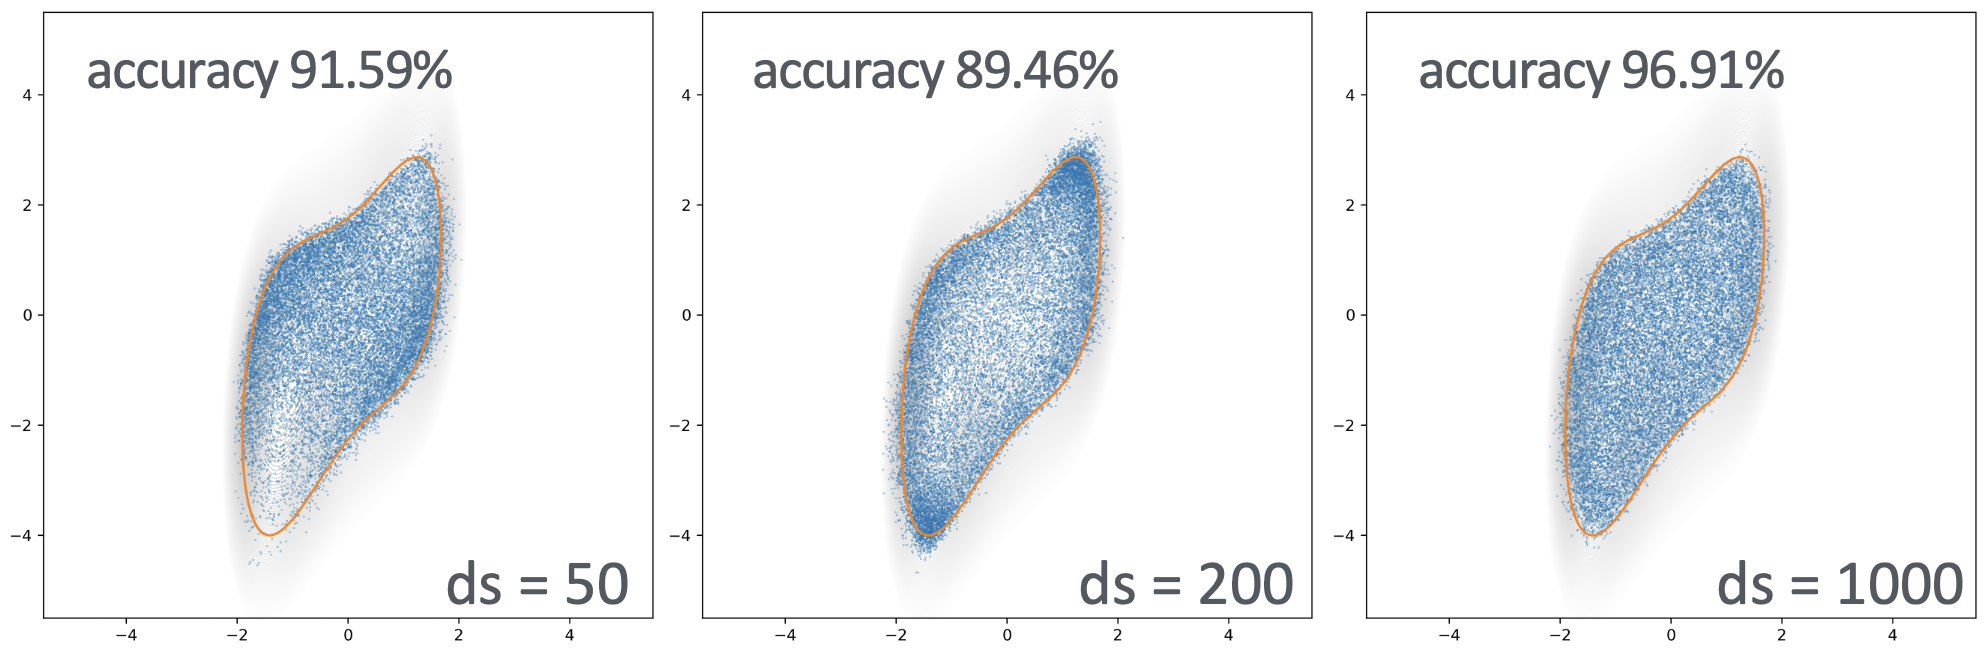
\includegraphics[width=0.9\linewidth]{images/accur_1.png}
    \caption{Pool generated from trained diffusion models, all with the same original data and thus same energy and contour level to replicate. Here we compare the results of three models with different diffusion steps. More results can be found in the \href{https://github.com/tommasoperitoree/CSM_Lab}{project} under ./resources/sampling$\_$results/conditioning/.}
    \label{fig:accur_1}
\end{figure}

Accuracy, which we have simply measured as the percentage of points whose energy falls within the threshold, is already at a good spot with as little as $50$ diffusion steps, which is actually the value used in the the paper. However the slight drop of accuracy for more diffusion steps (at $ds=200$) and then the bigger improvement at $ds=1000$, as well as the images itself suggests more in depth evaluation. In fact a mere accuracy benchmark seems to be inappropriate, as for little diffusion steps the distribution obtained is well within the bound but very closely resembles a normal distribution, which in the picture would be points evenly distributed inside a circumference around the origin with radius of $1$. It seems in fact that the model of $50$ diffusion steps barely starts to spread the distribution to reach the two spots in the upper-right and lower-left corners. Subsequently, the model with $ds=200$ seems to understand more the shape of the contour but overshoots the corners, making them densely populated and thus getting worse results in accuracy. Finally, only the highest diffusion steps number seems to allow for a truly evenly spread distribution. 

This suggested us to compare better the density of points in the generated pools. To do this we laid over our two-dimensional position space a grid of bins in order to obtain an histogram from the pool. The results are shown, for the same contour level, in fig. \ref{fig:den_1} where the absolute density is shown. 

\begin{figure}[ht]
    \centering
    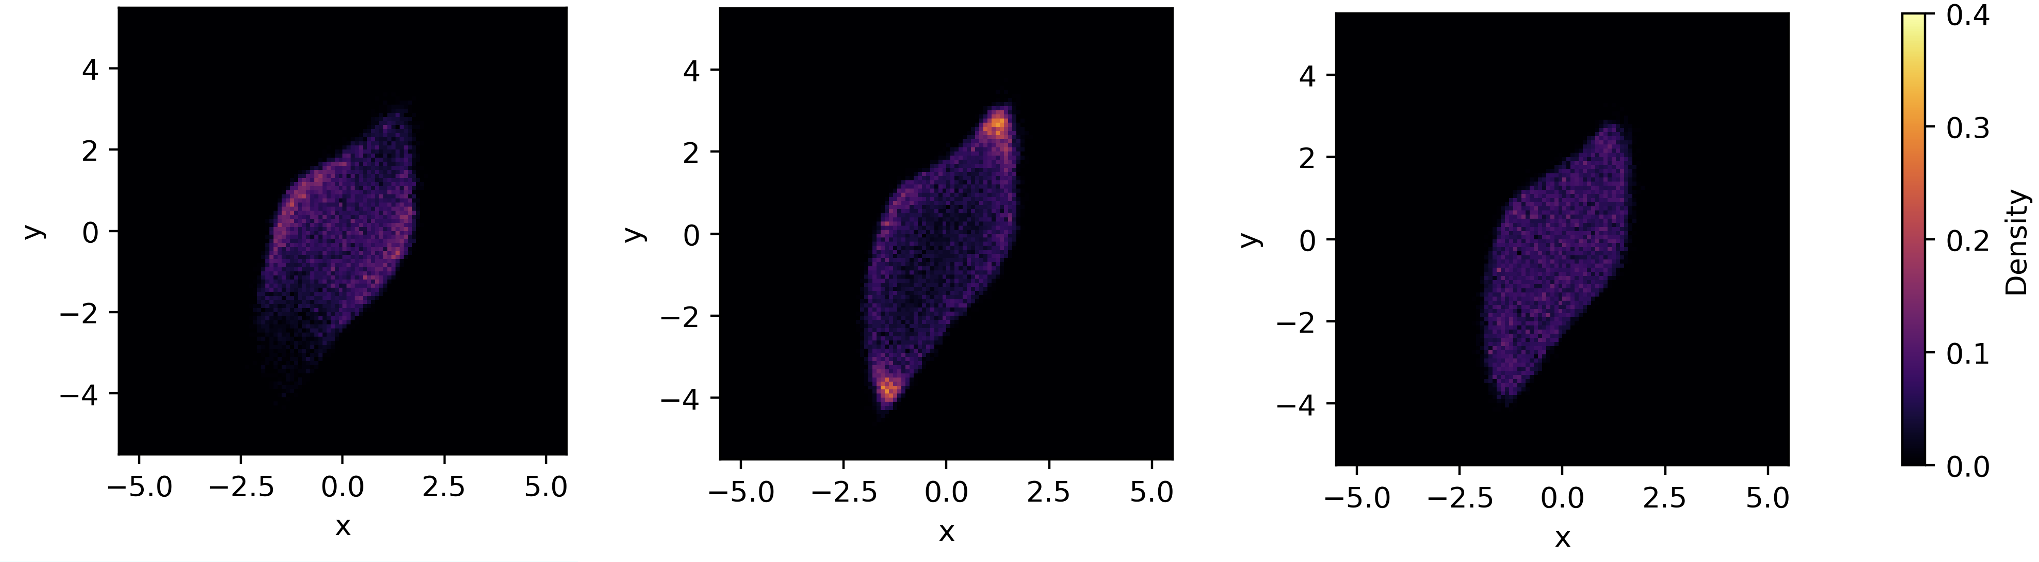
\includegraphics[width=\linewidth]{images/den_1.png}
    \caption{Density histograms of the final generated pools for different numbers of diffusion steps, again for $ds=50$, $200$, $1000$ from left to right. More results can be found in the \href{https://github.com/tommasoperitoree/CSM_Lab}{project} under ./resources/sampling$\_$results/conditioning/histograms/.}
    \label{fig:den_1}
\end{figure}

A further comparison was done (see fig. \ref{fig:den_diff_1}) by subtracting the generated pool bins from the ones of the original live set, the one generated from the NS algorithm and that was used to train the model. These visualization helps to make more evident what was mentioned above of the different behaviors of the model for different numbers of diffusion steps. That is, that the first under populates the corners, while the second overshoots them, and only with the last model do we achieved a truly uniform distribution. 

\begin{figure}[ht]
    \centering
    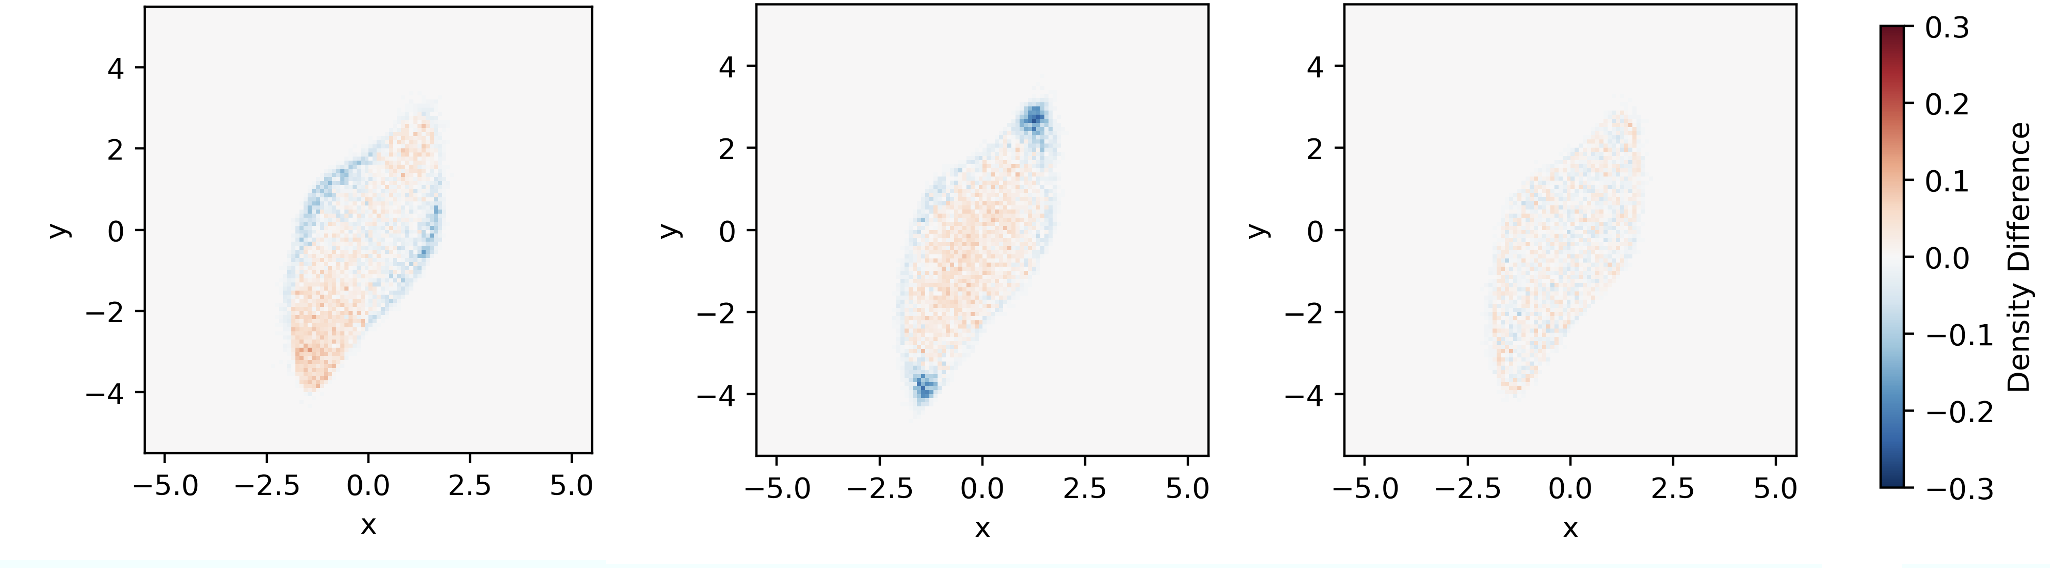
\includegraphics[width=\linewidth]{images/den_diff_1.png}
    \caption{Histograms showing density difference from the original live set of the final generated pools for different numbers of diffusion steps, again for $ds=50$, $200$, $1000$ from left to right. More results can be found in the \href{https://github.com/tommasoperitoree/CSM_Lab}{project} under ./resources/sampling$\_$results/conditioning/histograms/}
    \label{fig:den_diff_1}
\end{figure}

Of all of these results, there is more material to be found in the GitHub repository, together with animations that allow to compare also the evolution of the sampling. From the observation of these we confirmed that the lower number of diffusion steps either did not give enough time for the model to progress accurately or forced the model to infer the shape of the contour too quickly. 




\subsection{Mixed algorithm}

% missing a tiny intro

\subsubsection{Conditioning}

We said above that the standard Diffusion model was introduced with as input nodes the positional degrees of freedom plus one variable, time, to encode the progressive denoising from gaussian  to the target distribution. On top of that we can add a further node of input to condition the model with a value of energy. Interesting is the fact that the model does not know what that number represents, but simply takes it as a tag, additional info that we do not actually know how it uses. Nevertheless we wanted to evaluate the performance of the model depending on the presence of this feature. The range of energies that the potential (see eq. \ref{eq:pot}) gives from the maximum of our initial set of positions to the values reached when exploring the minima is about $U(x,y)\in[-3,30]$. This are numbers that the model would have a hard time working with, since usually a good range is $[0,1]$ for the operations that the network executes. Thus we implemented a scaling factor (together with translation) to always give reduced energy values in this range. 

\begin{figure}[ht]
    \centering
    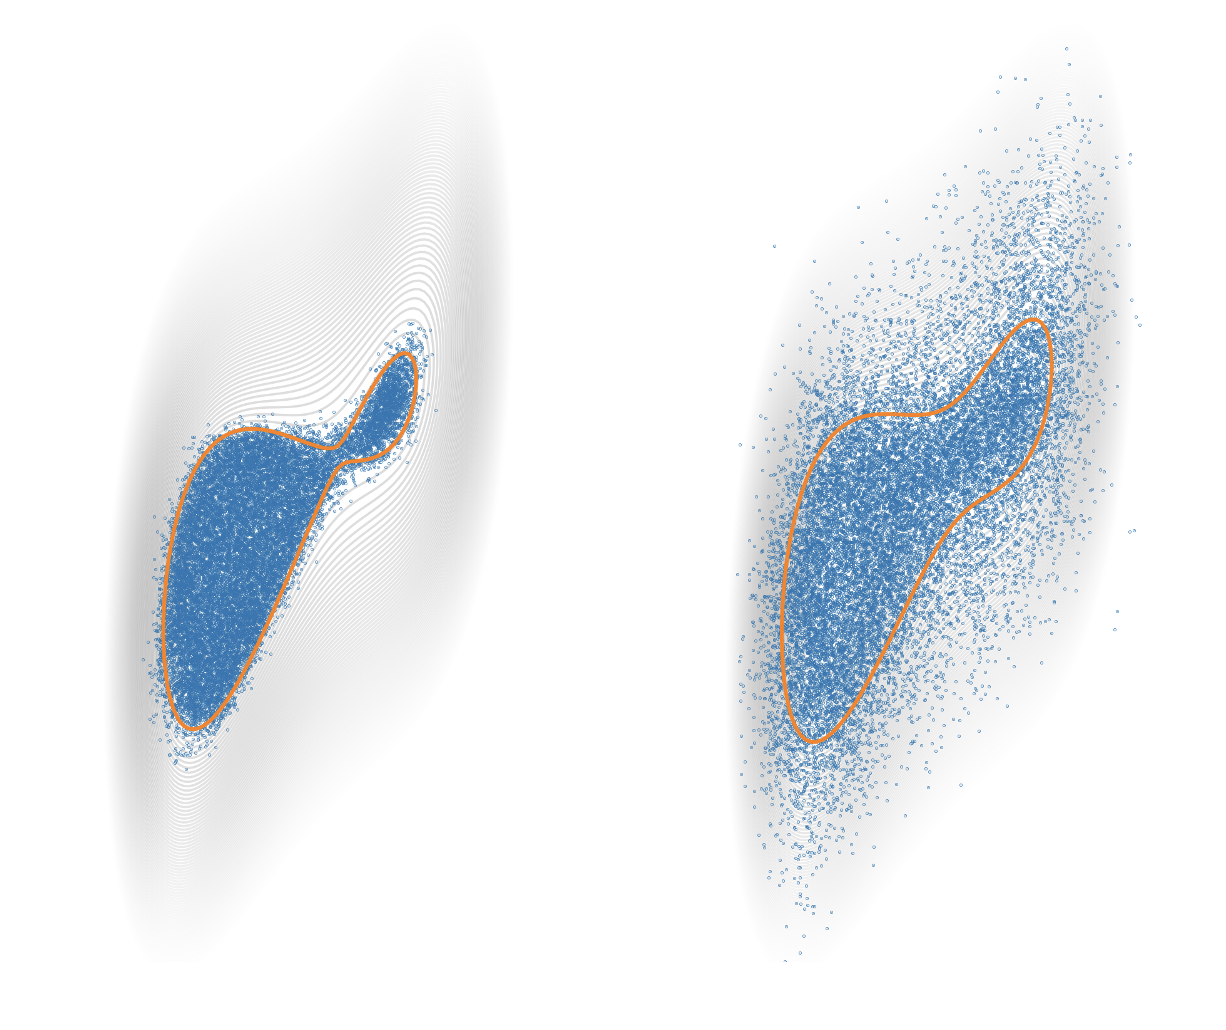
\includegraphics[width=.6\linewidth]{images/cond_last.png}
    \caption{Live set generated from model trained with conditioning (left) and without conditioning (right). This specifically is the second step of the mixed routine. More results can be found in the \href{https://github.com/tommasoperitoree/CSM_Lab}{project} under ./resources/mixed$\_$routine/last$\_$live$\_$samples/, compare conditioned with unconditioned images, named with stepX.5.png, where the X stands for the step number within the mixed algorithm.}
    \label{fig:cond_last}
\end{figure}

We tested the mixed algorithm to show how the conditioning might affect it. One result is shown in fig. \ref{fig:cond_last} where one can clearly see how if at the beginning the shape of the contour is easier to replicate, in the picture which is only the second training step, the conditioned model performs significantly better. On the GitHub repository one can find conditioned and unconditioned generated live sets (named stepX.5.png) to distinguish them from the results of the NS portion of the algorithm. 

Since we saw right from the beginning that conditioning the model had a huge impact on its performance, this is one of the things that we kept right away for the mixed algorithm.

\subsubsection{Multiple live sets to train}

Another hypothesis of feature to insert in our mixed algorithm was the feeding upon training of multiple live sets to the model. The way we integrated it was to give all the previous live sets reached through NS to the model. Since the training was always independent from the previous, the values of the conditions were given after scaling in order to put the highest energy at $u=1$ and the lowest at $u=0$. In fig. \ref{fig:cond_comp} we can see this feauture put in use (image to the left) right next to the algorithm executed exactly with the same parameters, just with training on a single live set. The picture shows how the model seems to in fact be helped by training with more live sets. This can be seen throughout the execution, also at different levels of the potential (see GitHub for more pictures). 

\begin{figure}[ht]
    \centering
    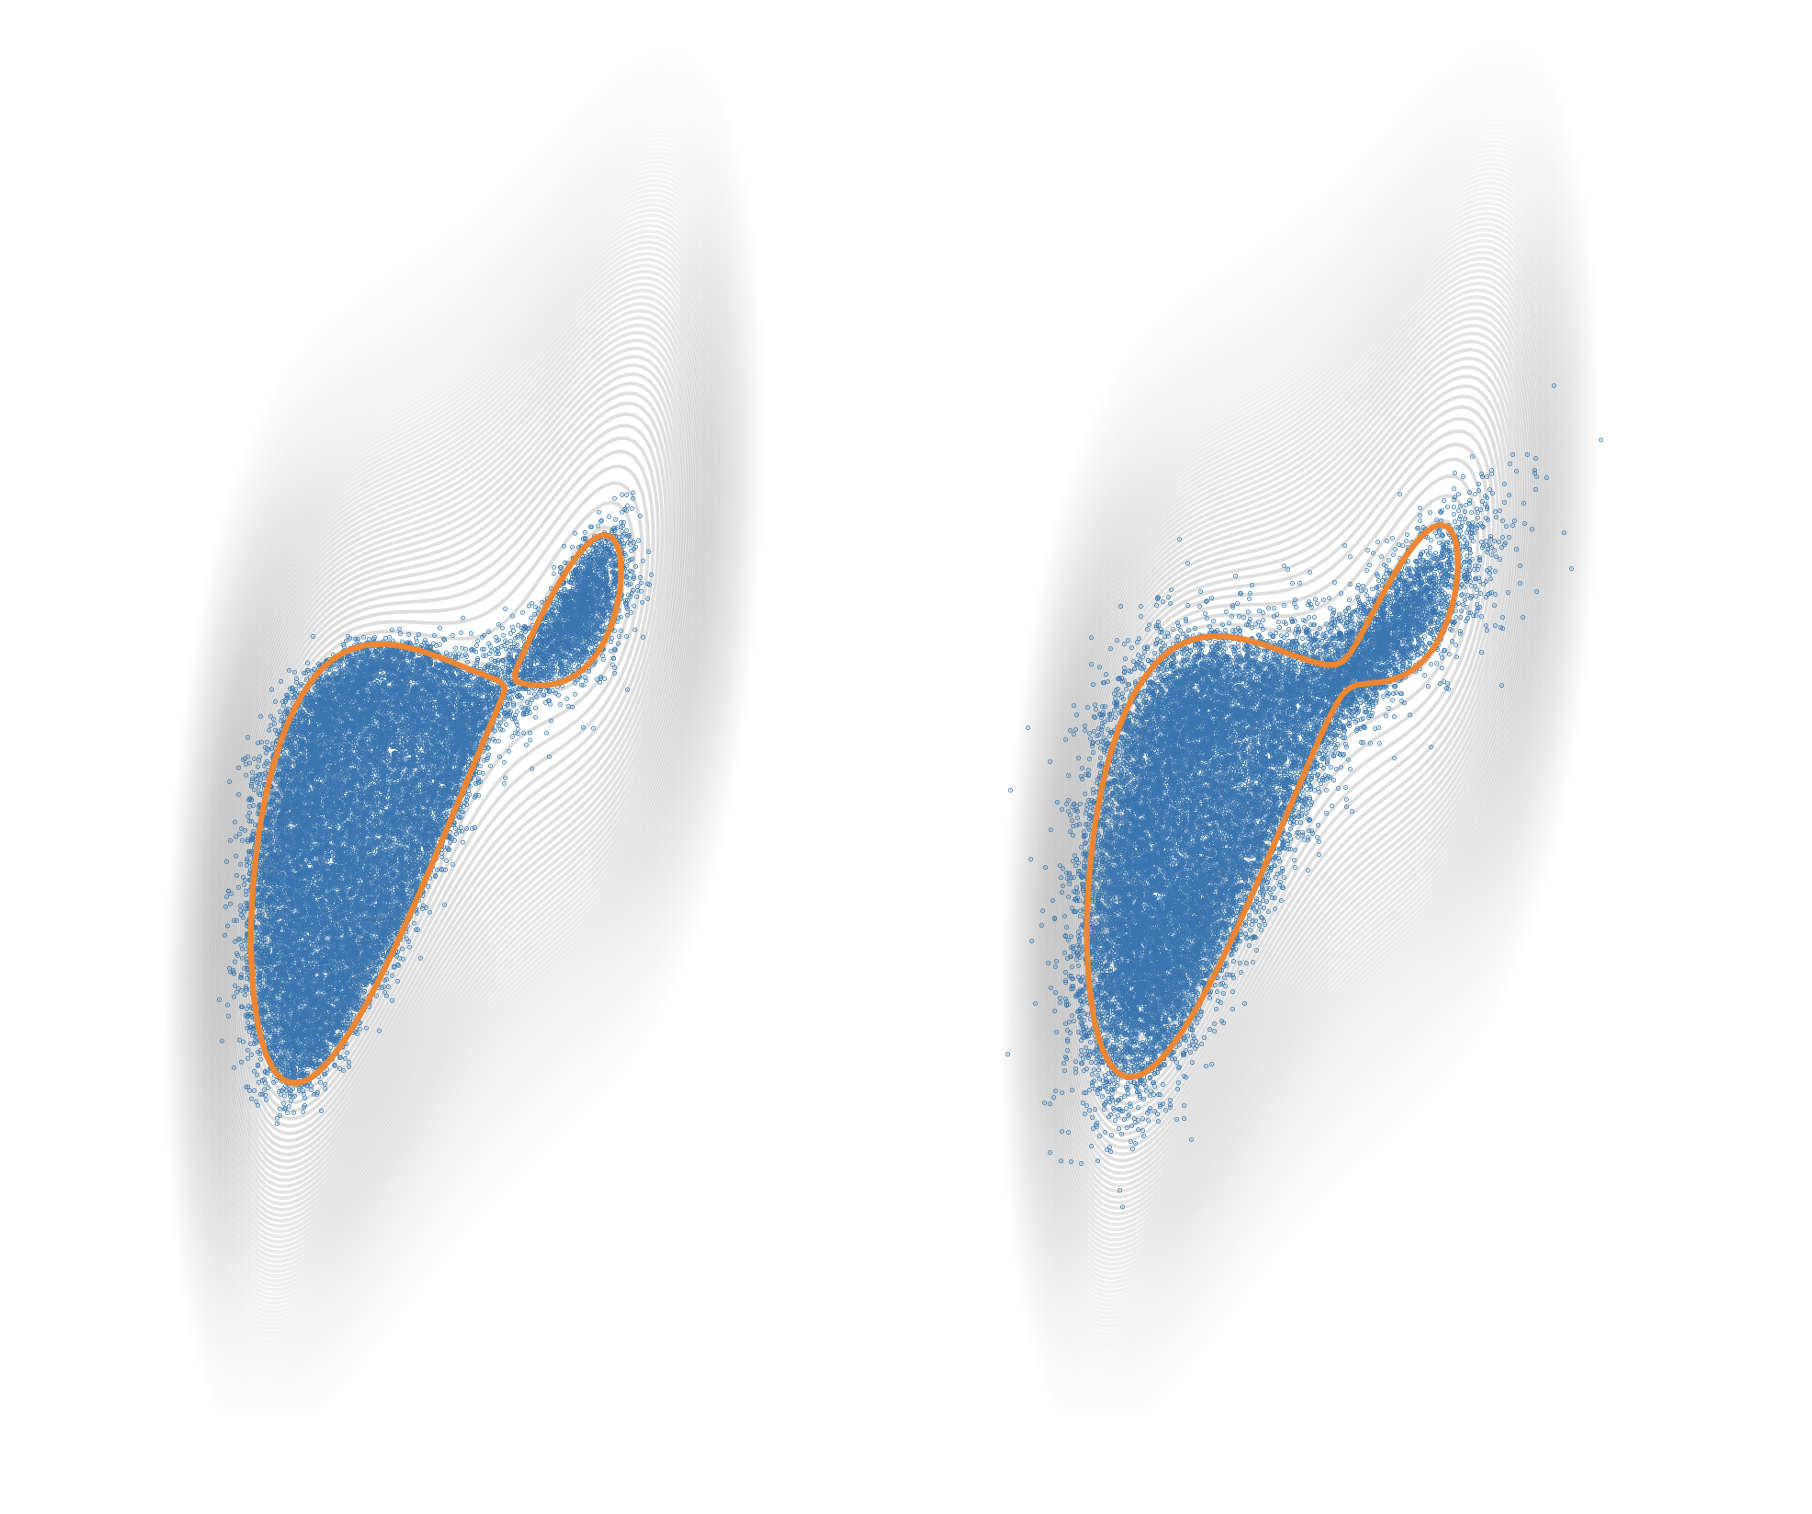
\includegraphics[width=.6\linewidth]{images/cond_comp.png}
    \caption{Comparing performances of models trained with conditioning from all previous live sets (left) or only with one (right). More results can be found in the \href{https://github.com/tommasoperitoree/CSM_Lab}{project} under ./resources/mixed$\_$routine/ compare last live sample with all live samples directories.}
    \label{fig:cond_comp}
\end{figure}

With more live sets, training takes longer execution time, so we explored also the different it made to disregard more live sets further in the algorithm. That is, for example, training with the last three live sets, rather than all the previous ones. The performances of the model trained this way seem to not be affected too much, and execution time is contained. 

\subsubsection{Extrapolation}

\begin{figure}[ht]
    \centering
    
\includegraphics[width=.8\linewidth]{images/extr_comp.png}
    \caption{Testing performances of extrapolation. Model trained with conditioning from all previous live sets. On the left is the live set used to train the model, on the left is the generated set when asked to sample at the energy in orange. More results of extrapolation can be found in the \href{https://github.com/tommasoperitoree/CSM_Lab}{project} for different mixed algorithm details (conditioning, number of live sets used for training, etc.).}
    \label{fig:extr_comp}
\end{figure}

Finally a big hope we could have with our algorithm is that the model pick up enough knowledge on the behavior of the potential to extrapolate. That is, we wish to ask our model to generate a live set whose energy threshold is slightly lower than the lowest energy of the live sets given to train on. To test this, we let some final NS steps after the use of the last trained model. This brought the live set to a lower energy than what the model had been trained on. And then we used the same model, sampling on it but asking for the energy reached by that final NS step. 

The result can be seen in fig. \ref{fig:extr_comp} and the model used was the one that thus far had been performing the best. However it is evident that the model does not produce something very far from the live set it was trained on, despite having been asked for a lower energy. This behavior did not surprise us too much as extrapolation beyond the train data is something these networks struggle to do in general.

\subsubsection{Performances}

Finally, since so far we have observed that the mixed scheme, as hoped, does help the NS algorithm by exploiting the generative power of the DM, we now would like to understand if this is actually an improvement from the original algorithm. The problem of how to evaluate this improvement is not obvious to solve. One parameter is for sure mere execution time, which for consistency I have benchmarked on a single portable station, executing one instance of mixed algorithm at a time. A second parameter is a count of "global steps", that is every time a nested sampling step or equivalently one position from the generated live set is used, then the count is increased. This is a particular parameter as for NS, a single count has moved all the positions several steps (the number chosen to decorrelate), while for the model portion, a step has moved a single point (by replacing it with a new from the generated pool). Finally an important parameter to observe is the number of energy function calls during the execution. In fact, the potential we used is a simple 2D one, while for interesting use cases, the potential could be 3D and with many bodies involved (as it is in normal matter interaction, for example with a Lennard-Jones potential). In these scenarios, calculating the energy of the system given all the positions involved can be a more demanding task computationally. Since throughout the algorithm this is a computation repeated over and over, the cost could be determinant on the total execution time. 

We will use to compare the mixed scheme to the sole NS algorithm by showing the energy reached by the live set as function of these presented parameters. First off, the graphs of the mixed scheme alone can be found in fig. \ref{fig:mx_benchm}, where each graph has been color coded to show the portion of the algorithm using NS and the portion sampling from the model generated pool. 

\begin{figure}[ht]
    \centering
    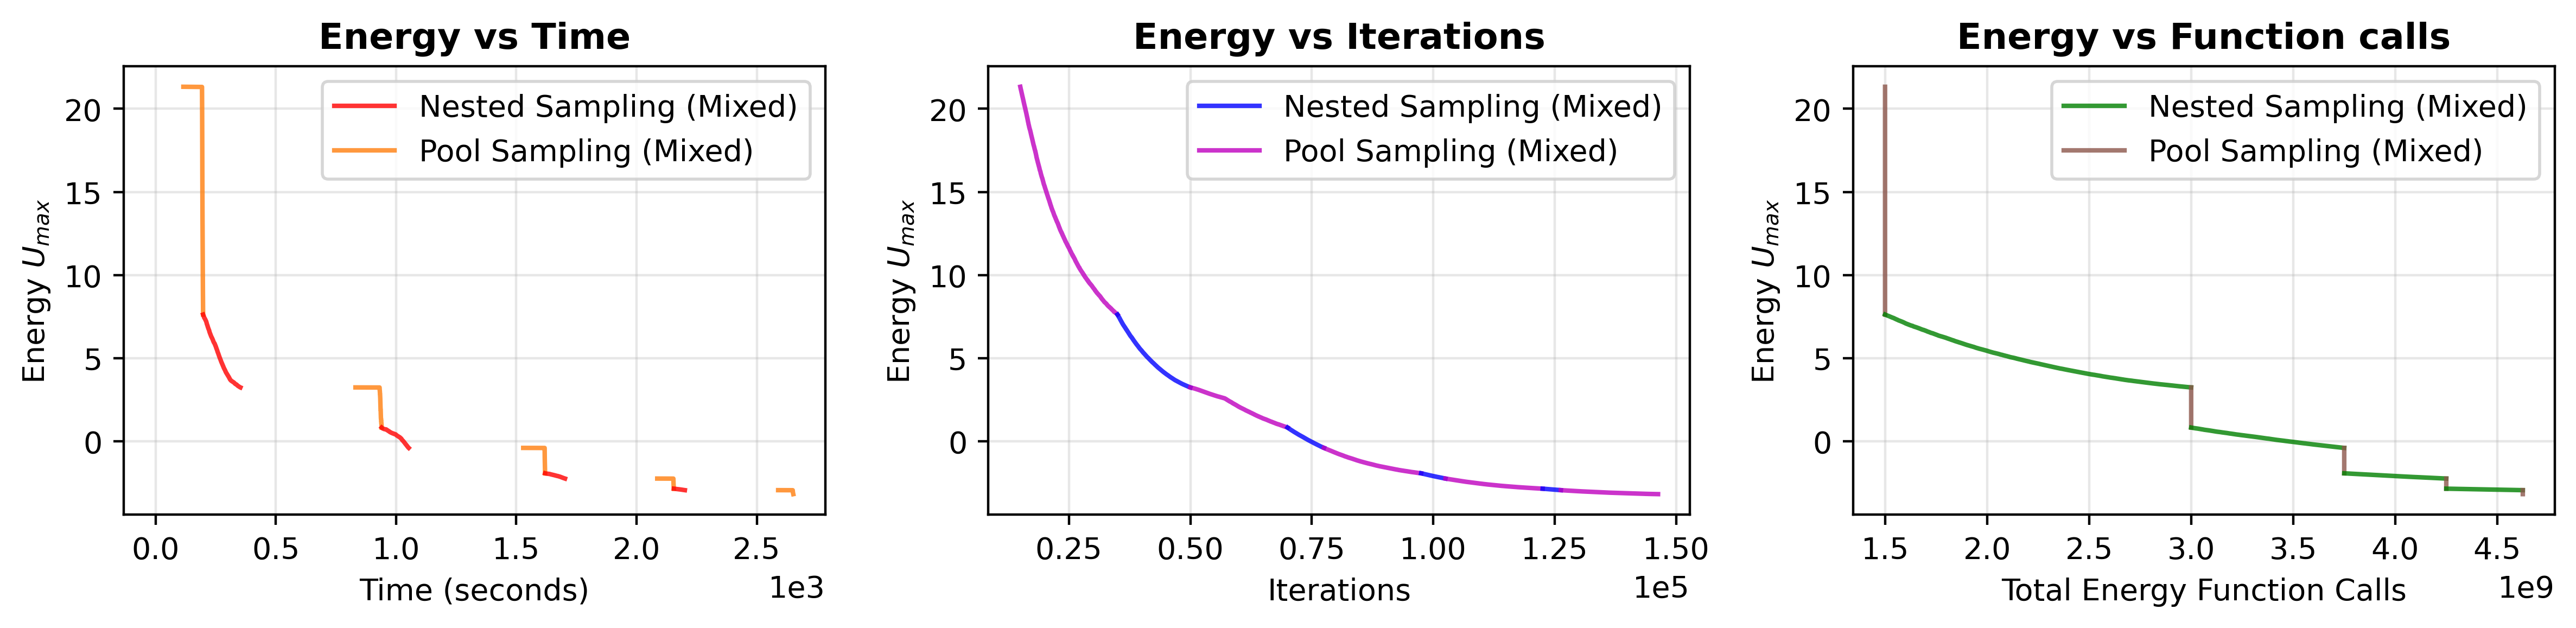
\includegraphics[width=\linewidth]{images/mx_benchm.png}
    \caption{Benchmark graphs of the mixed scheme, looking at energy scaling with execution time, global steps and energy function calls.}
    \label{fig:mx_benchm}
\end{figure}

These graphs by themselves show something interesting, even before comparing them to the NS algorithm performances. First the energy vs. time graph, where the algorithm is initiated from a pre-saved NS reached live set. Thus the first section of the graph, before the horizontal line begins, is the time dedicated to training. Then the horizontal portion is the sampling, before the points start to be used, where the energy of the live set suddenly drops, in almost no time, sign of a very efficient algorithm. Then the NS portion is evidently slower at going down the potential. This trend is evident also in the later steps of the mixed scheme. Secondly, the energy vs iterations graph shows a quite consistent trend, despite the particularity of the parameter that we mentioned above: having defined the single iteration for NS as a move of all points, and for the pool sampling as the use of a single point, the fact that the different portions of the curve are comparable suggests that the use of the model generated points is more efficient at taking the live set down the potential. Our hypothesis on the fact that at the end of the curve this difference is not so evident is that with the tighter energy contours, more generated points are discarded quickly for having gone outside new energy threshold. Finally, the graph energy vs function calls is very expressive. The portion where we use the model uses far less calls of the energy function to take down the energy of the live set.

\begin{figure}[ht]
    \centering
    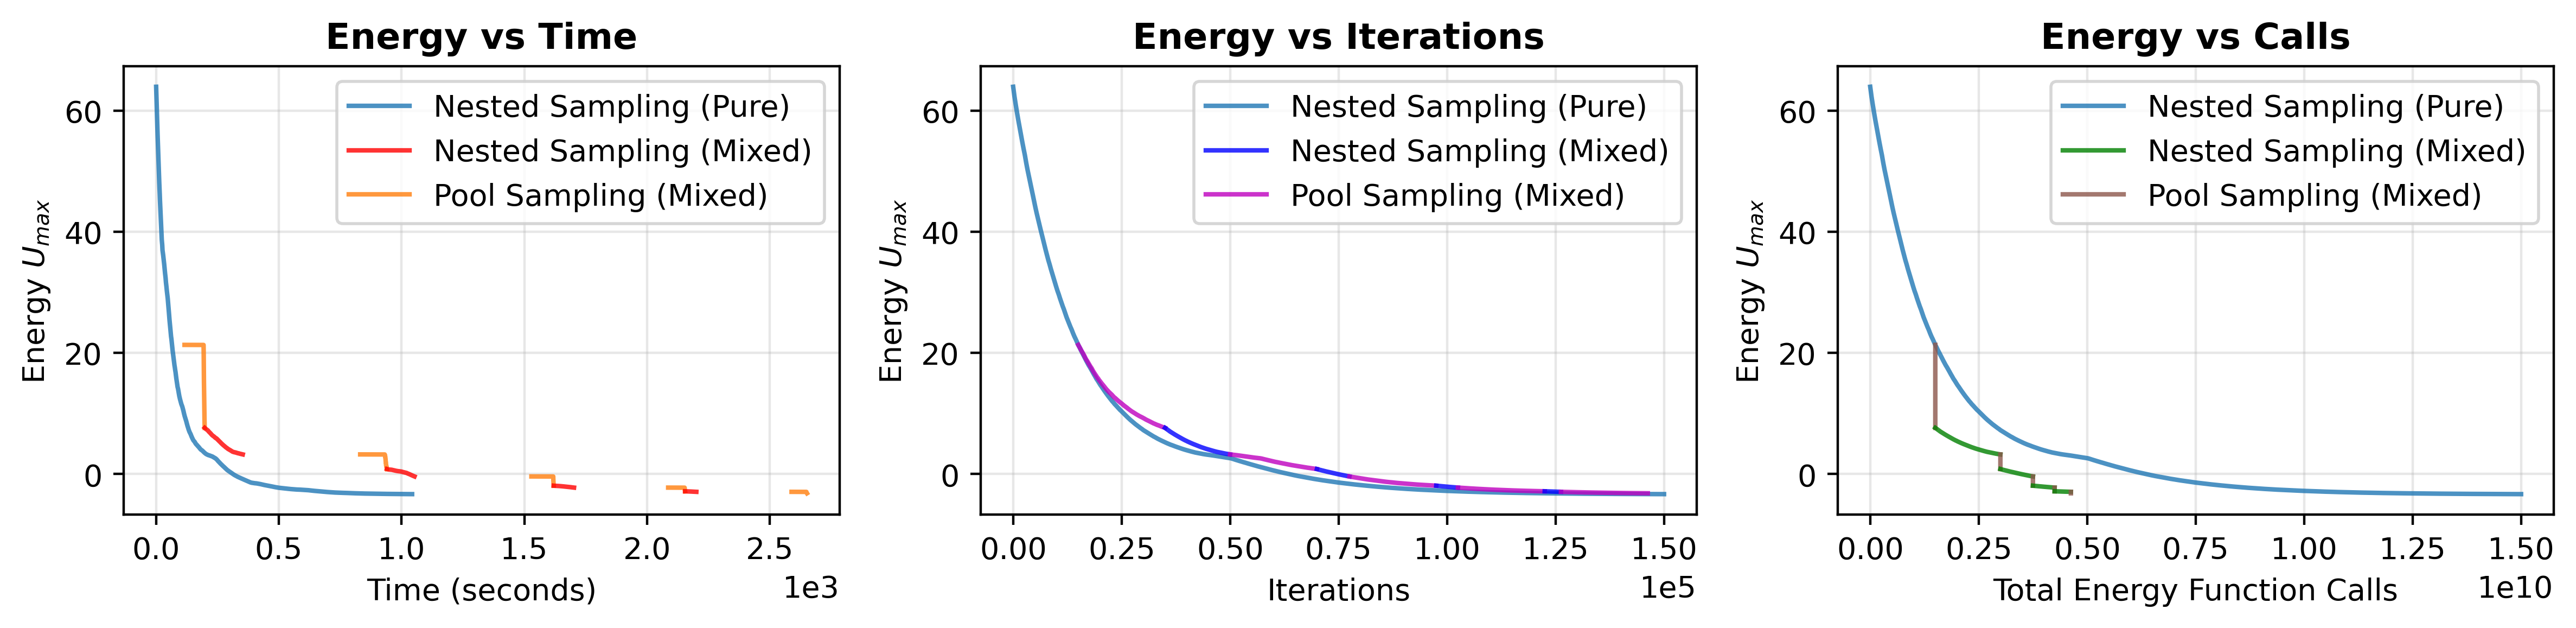
\includegraphics[width=\linewidth]{images/benchm_comp.png}
    \caption{Benchmark comparison of the Nested Sampling algorithm by itself to the Mixed scheme.}
    \label{fig:benchm_comp}
\end{figure}

Now we can compare in fig. \ref{fig:benchm_comp} the above graphs with the performances of the NS algorithm by itself. The first shows how execution time is severely affected by the time it takes to train and then sample the model. This depends strongly on the fact that these operations require the graphics cards of the machine used that were definitely not optimized for these tasks, while the NS algorithm only needs to run on CPUs. Furthermore, the iterations graph are pretty closely resembling each other. Finally, the last graph shows again how the energy function needs to be called a lot less when executing the model portion of the mixed scheme compared to NS steps. 

\newpage \section{Conclusions}

The study demonstrates that diffusion models, when conditioned on energy values and trained on successive live sets, can complement the nested sampling algorithm by generating uncorrelated and uniformly distributed configurations. Conditioning was shown to significantly enhance performance, and training on multiple live sets further improved the reproduction of energy contours. However, attempts at extrapolation beyond trained energy thresholds confirmed a general limitation of generative models, as the diffusion network struggled to generalize to unseen energy levels.

The benchmark analysis provided additional insights into the practical effectiveness of the mixed algorithm. While training and sampling with the diffusion model incurred a substantial overhead in execution time — primarily due to GPU-intensive operations — the algorithm consistently required fewer energy function evaluations than standard nested sampling. This is particularly relevant for applications involving high-dimensional or many-body potentials, where energy evaluations dominate computational cost. Furthermore, the analysis of global steps suggested that diffusion-generated points can accelerate the descent in energy, even though the advantage diminishes at lower energy thresholds due to higher rejection rates.

Overall, the mixed algorithm shows promising potential for improving the efficiency of sampling energy landscapes. The results indicate that while execution time remains a bottleneck under the present implementation, the significant reduction in energy function calls highlights the method's scalability and possible advantages in more demanding scenarios. Future refinements should focus on optimizing model training efficiency and improving robustness against extrapolation, paving the way for practical applications of generative-enhanced nested sampling in complex physical systems, which this study was not able to adress.



\newpage \bibliographystyle{unsrt} \bibliography{main}

\end{document}